\documentclass[aspectratio=169,11pt]{beamer}
\usetheme[secheader]{Boadilla}
\usecolortheme{seahorse}
\usepackage[T1]{fontenc}
\usepackage[utf8]{inputenc}
\usepackage{lmodern,amsmath,amssymb,booktabs,graphicx}
\setbeamercolor{frametitle}{fg=black,bg=black!5}
\setbeamersize{text margin left=3mm,text margin right=3mm}
\setbeamerfont{caption}{size=\scriptsize}
\setbeamertemplate{caption}[numbered]
\title[Hidden-state evolution in Chronos-2]{Measuring Hidden-State Evolution\\in Chronos-2}
\subtitle{Methods of Sequential Data}
\author[N. Aleksandrov et al.]{Nikita Aleksandrov \quad Ilya Lobanov \quad Namig Damirov}
\institute[Skoltech]{Skolkovo Institute of Science and Technology}
\date{October 26, 2026}
\newcommand{\R}{\mathbb{R}}
\begin{document}

\begin{frame}
\titlepage
\end{frame}

\section{Problem statement}
\subsection{Research question}
\begin{frame}{Problem statement}
A time-series foundation model processes a window of observations and forms an internal representation $h_t$.
\[
 x_{q_t-C+1:q_t}\;\xrightarrow{\text{frozen model}}\;h_t.
\]
As the observation window moves, the internal representation changes.
\vspace{3mm}

\textbf{Question:} can a simple fixed model predict that change?
\[
 \widehat h_{t+k}=F_k(h_t).
\]
We test the required model complexity, the useful forecast horizon and alternative explanations for predictability.
\end{frame}

\subsection{Related work}
\begin{frame}{Literature overview}
\begin{table}
\centering
\renewcommand{\arraystretch}{1.35}
\begin{tabular}{p{.20\textwidth}p{.32\textwidth}p{.33\textwidth}}
\toprule
Representation & Snapshot / across depth & Series-time dynamics \\
\midrule
Native, frozen & Wili\'nski et al.\newline Internal Semantics\newline Transformer Dynamics & \textbf{Our question:}\newline predictive transitions in native TSFM states \\
\midrule
Trained for prediction & --- & LatentTSF\newline EIDOS / LaT-PFN\newline MIRA \\
\bottomrule
\end{tabular}
\end{table}
\vspace{2mm}
Depth indexes network layers. Series-time indexes successive observation windows.
We study native states without training the backbone for a new dynamics objective.
\end{frame}

\section{Experimental setup}
\subsection{Data and states}
\begin{frame}{Synthetic data generation}
\begin{columns}[T,onlytextwidth]
\begin{column}{.48\textwidth}
\textbf{Lorenz: convection model}
\[
\begin{aligned}
\dot x&=\sigma(y-x),\\
\dot y&=x(\rho-z)-y,\\
\dot z&=xy-\beta z.
\end{aligned}
\]
$\sigma=10$, $\rho=28$, $\beta=2.667$.
\end{column}
\begin{column}{.48\textwidth}
\textbf{R\"ossler: chaotic oscillator}
\[
\begin{aligned}
\dot x&=-y-z,\\
\dot y&=x+ay,\\
\dot z&=b+z(x-c).
\end{aligned}
\]
$a=0.2$, $b=0.2$, $c=5.7$.
\end{column}
\end{columns}
\vspace{4mm}
We observe the first coordinate $x$ and keep the system parameters fixed across series. Initial conditions differ between series.
\vspace{3mm}

\scriptsize Source: Gilpin (2021), \texttt{dysts}, \url{https://arxiv.org/abs/2110.05266}.
\end{frame}

\begin{frame}{Datasets}
\begin{figure}
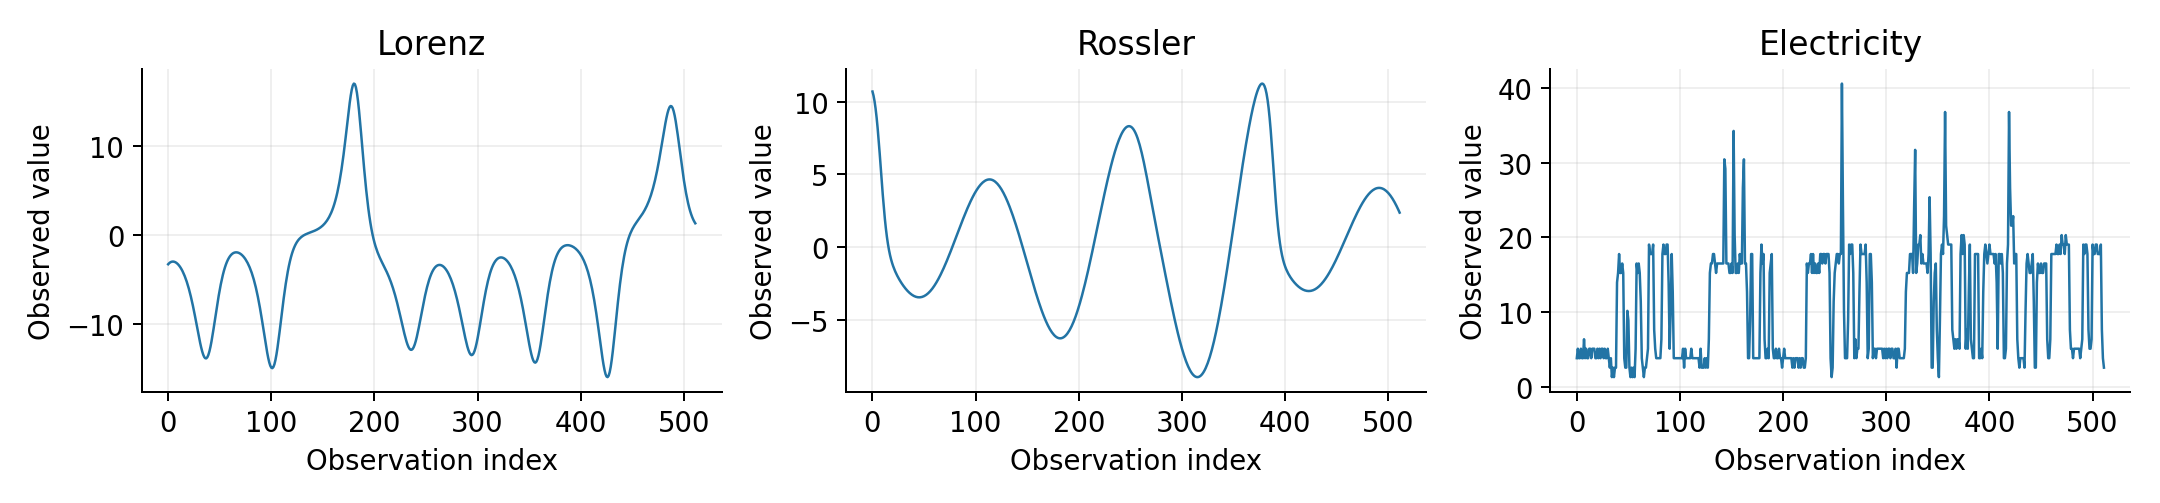
\includegraphics[width=.93\textwidth]{images/dataset_examples.png}
\caption{The first 512 observations of the first training series in each dataset. Values use each dataset's original scale.}
\end{figure}
\small
\begin{itemize}
\item \textbf{Lorenz and R\"ossler:} observe $x$ from the systems on the previous slide.
\item \textbf{Electricity:} quarter-hour meter readings, 96 observations per day.
\item \textbf{Controls:} $x_{t+1}=\phi x_t+\epsilon_t$, independent Gaussian $\epsilon_t$. AR(1): $\phi=0.9$; white noise: $\phi=0$.
\end{itemize}
\scriptsize Electricity source: GIFT-Eval, \url{https://arxiv.org/abs/2410.10393}.
\end{frame}

\begin{frame}{Hidden-state extraction}
\begin{columns}[T,onlytextwidth]
\begin{column}{.53\textwidth}
\begin{itemize}
\item Chronos-2: 119.5M parameters
\item 12 blocks, 12 attention heads
\item Hidden width 768, FFN width 3072
\item Input patches: 16 observations
\item Model context limit: 8192
\item Our context: 512; shift: 16
\item State: middle block 5 (6th of 12), last observed patch
\end{itemize}
\end{column}
\begin{column}{.43\textwidth}
\[
\begin{aligned}
h_t&=E_5(x_{q_t-511:q_t}),\\[2mm]
h_{t+1}&=E_5(x_{q_t-495:q_t+16}).
\end{aligned}
\]
Adjacent windows share 496 observations.
\end{column}
\end{columns}
\vspace{5mm}
We recompute each state from its window. The encoder does not carry a recurrent state between windows.
\end{frame}

\subsection{Models}
\begin{frame}{Prediction tasks}
\textbf{Input:} the current hidden state $h_t$. \textbf{Target:} $h_{t+k}$.
\vspace{2mm}

Direct prediction fits a separate map for each horizon:
\[
 \widehat h_{t+k}=F_k(h_t).
\]
Recursive prediction fits one transition and applies it $k$ times:
\[
 \widehat h_{t+1}=F(h_t),\qquad \widehat h_{t+k}=F^{\circ k}(h_t).
\]
The main grid uses recursive prediction at $k=1,4,16,64,256$.
One base step advances the input window by 16 observations.
\end{frame}

\begin{frame}{Transition models}
For the recursive task, normalize $z=(h-\mu)/s$ and predict
\[\widehat h_{t+k}=\mu+s\odot F^{\circ k}(z_t).\]
\[
 f_\theta(z)=W_2\tanh(W_1z+a)+b.
\]
\begin{table}
\centering
\begin{tabular}{ll}
\toprule
Model & One analysis step \\
\midrule
Ridge & $\widehat h_{t+1}=Ah_t+b$ \\
MLP & $z_{t+1}=f_\theta(z_t)$ \\
Residual & $z_{t+1}=z_t+f_\theta(z_t)$ \\
Neural ODE & $\dot z=f_\theta(z)$, integrate over $\Delta t=1$ \\
\bottomrule
\end{tabular}
\end{table}
\begin{itemize}
\item Neural models share a $768\to256\to768$ Tanh architecture, with separate fitted weights.
\item Fit neural models on four-step segments. Select epochs using validation $k=4$.
\item Baselines: the training-target mean and persistence, $\widehat h_{t+k}=h_t$.
\end{itemize}
\end{frame}

\subsection{Evaluation}
\begin{frame}{Evaluation protocol}
\begin{table}
\centering
\begin{tabular}{ll}
\toprule
Parameter & Value \\
\midrule
Primary datasets & Lorenz, R\"ossler, electricity \\
Training / validation & 8 / 4 separate series per dataset \\
Neural initialization seeds & 3 for every model and dataset \\
Recursive horizons $k$ & 1, 4, 16, 64, 256 \\
One analysis step & 16 original observations \\
ODE integration & RK4, 4 substeps during training and rollout \\
\bottomrule
\end{tabular}
\end{table}
\begin{itemize}
\item All models and all five horizons use the same reporting starts.
\item Fit scaling and PCA on training data only.
\item All reported scores use validation data. Final test partitions remain closed.
\end{itemize}
\end{frame}

\begin{frame}{Accuracy metrics}
For each validation series,
\[
R^2=1-\frac{\sum_t\|\widehat h_{t+k}-h_{t+k}\|_2^2}
                 {\sum_t\|h_{t+k}-\bar h_{\mathrm{train},k}\|_2^2}.
\]
\begin{itemize}
\item $R^2=0$: the training-target mean baseline
\item $R^2<0$: worse than that baseline
\item Average scores equally across validation series
\end{itemize}
\vspace{2mm}
We also check coordinate-standardized and whitened PCA scores.
For long trajectories, we compare distributions, ACF and PSD in a training-fitted projection.
\end{frame}

\section{Results}
\subsection{Recursive prediction}
\begin{frame}{Short-horizon prediction}
\begin{table}
\centering
\begin{tabular}{lrrrr}
\toprule
Dataset & Ridge $k=1$ & MLP $k=1$ & Ridge $k=4$ & MLP $k=4$ \\
\midrule
Lorenz & 0.941 & 0.913 & 0.658 & 0.840 \\
R\"ossler & 0.999 & 0.997 & 0.997 & 0.996 \\
Electricity & 0.509 & 0.441 & 0.418 & 0.316 \\
\bottomrule
\end{tabular}

\caption{Validation $R^2$ on common starts. Every $k=4$ forecast applies the fitted transition four times. Neural columns average three seeds.}
\end{table}
\begin{itemize}
\item On Lorenz, MLP improves $k=4$ from 0.658 to $0.840\pm0.006$ across seeds.
\item Ridge is strongest on electricity under the tested budget.
\item Near-perfect R\"ossler scores require the recurrence and timescale caveats.
\end{itemize}
\end{frame}

\begin{frame}{Recursive prediction through 256 steps}
\begin{figure}
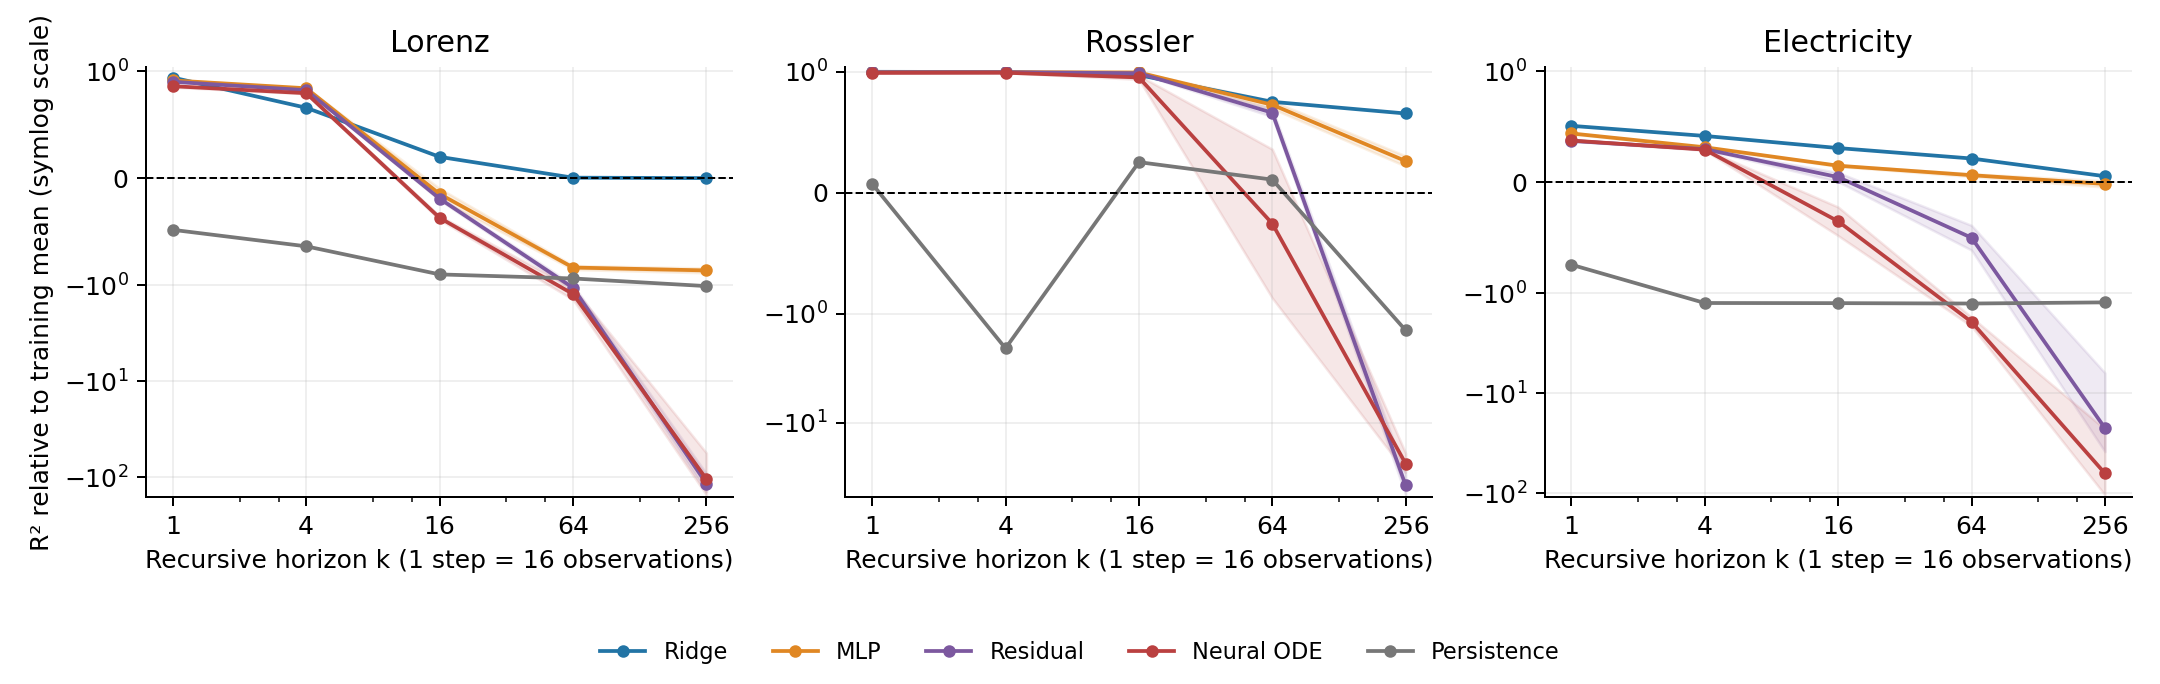
\includegraphics[width=\textwidth]{images/consistent_horizons.png}
\caption{$R^2$ versus horizon $k$. One step is 16 observations. Neural shading shows one seed standard deviation. The vertical scale is symmetric logarithmic.}
\end{figure}
\small
At $k=256$, ridge retains 0.655 on R\"ossler, approximately zero on Lorenz and 0.055 on electricity.
\end{frame}

\begin{frame}{Long trajectories in hidden-state space}
\begin{figure}
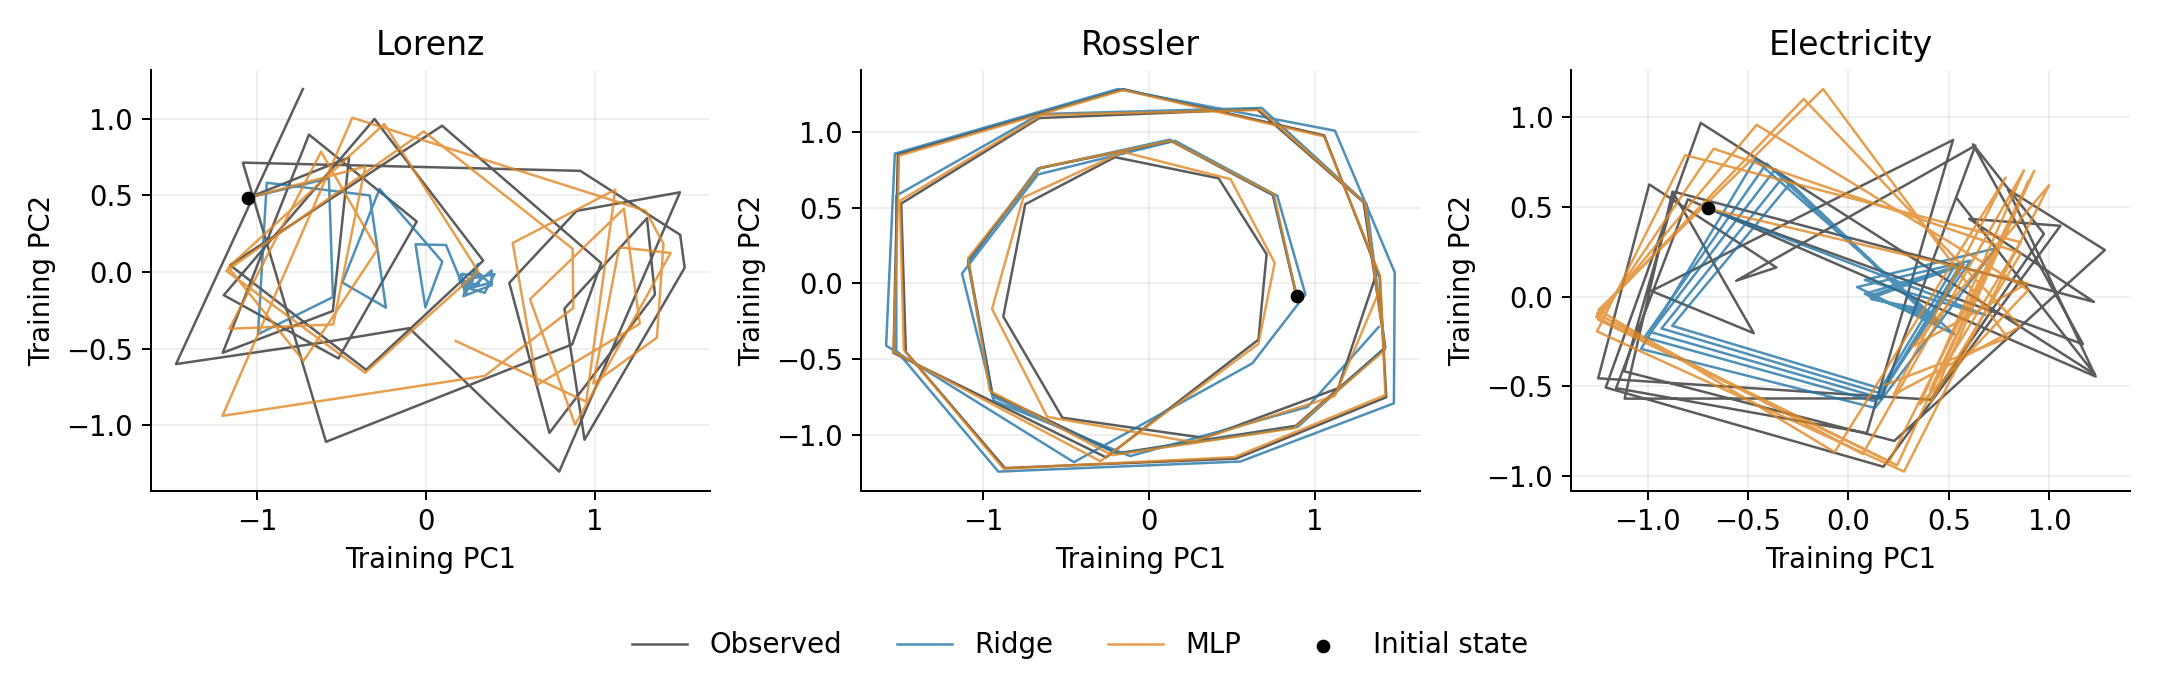
\includegraphics[width=.87\textwidth]{images/trajectory_prefix32.png}
\caption{First 32 steps of the 256-step rollouts in training PC1--2. First fixed sampled start; MLP seed 2026. The dot marks the start. Statistics use all 256 steps.}
\end{figure}
\small
Ridge approaches a nearly constant state on Lorenz and electricity. MLP keeps varying but loses alignment with the observed trajectory.
These are diagnostic observations in a projection, not a recovered physical attractor.
\end{frame}

\begin{frame}{Why the linear rollouts differ}
For a fixed point $h^*=Ah^*+b$, a linear rollout satisfies
\[
 \widehat h_{t+k}-h^*=A^k(h_t-h^*).
\]
\begin{table}
\centering
\begin{tabular}{lll}
\toprule
Dataset & Spectral radius $\rho(A)$ & Consequence \\
\midrule
Lorenz & 0.971 & Strong asymptotic contraction \\
R\"ossler & 0.99986 & Oscillations decay much more slowly \\
Electricity & 0.99634 & Eventual contraction \\
\bottomrule
\end{tabular}
\end{table}
\small
All three radii are below one. The fixed affine maps converge asymptotically.
MLP can keep varying, but its four-step training loss does not require correct phase through 256 steps.
\end{frame}

\begin{frame}{Long-rollout metrics}
For predicted and observed paths, use training PCs $U$ and scales $\Lambda$.
Let $\xi=\Lambda_8^{-1/2}U_8^\top(h-\mu)$.
\[
 D_{\mathrm{SW}}=\left[\frac1{32}\sum_{j=1}^{32}
 W_2^2\!\left(\{u_j^\top\widehat\xi\},\{u_j^\top\xi\}\right)\right]^{1/2}.
\]
\[
 D_{\mathrm{ACF}}=\frac18\sum_{p=1}^2\sum_{\ell\in\{1,4,16,64\}}
 |\widehat\rho_p(\ell)-\rho_p(\ell)|,\qquad
 D_{\mathrm{PSD}}=\frac{\|\widehat P-P\|_F}{\|P\|_F}.
\]
\small
$u_j$ are fixed unit directions. SW pools the last 128 states; ACF and normalized PSD use PC1--2 over the full 256-step path.
Lower is better. These finite-path metrics do not prove recovery of an invariant measure.
\end{frame}

\begin{frame}{Distribution and temporal statistics}
\begin{table}
\centering\small
\begin{tabular}{llrrr}
\toprule
Dataset & Model & SW & ACF error & PSD error \\
\midrule
Lorenz & Ridge & 0.989 & 0.071 & 0.621 \\
 & MLP & 0.096 & 0.021 & 0.305 \\
R\"ossler & Ridge & 0.450 & 0.047 & 0.106 \\
 & MLP & 0.046 & 0.016 & 0.085 \\
Electricity & Ridge & 0.833 & 0.105 & 0.411 \\
 & MLP & 0.331 & 0.117 & 0.454 \\
\bottomrule
\end{tabular}

\caption{Finite 256-step forecasts from the same 16 starts per validation series. SW: sliced Wasserstein distance in whitened PC8 over the last 128 states. ACF and PSD use PC1--2. Lower is better.}
\end{table}
\begin{itemize}
\item On Lorenz and R\"ossler, MLP matches these statistics better than ridge, despite worse long-horizon pointwise $R^2$.
\item A pooled distribution match alone does not establish temporal dynamics.
\end{itemize}
\end{frame}

\subsection{Controls}
\begin{frame}{Forecasting the input, then encoding it}
Use the observed context $w_t$ and a predicted continuation $\widehat v_{t,k}$:
\[
 \widetilde h_{t+k}=E_5\!\left(\operatorname{tail}_{512}[w_t,\widehat v_{t,k}]\right).
\]
\begin{table}
\centering\small
\begin{tabular}{llrrr}
\toprule
Dataset & Ridge & MLP & Chronos & Last value \\
\midrule
Lorenz & 0.612 & 0.810 & -0.067 & -0.306 \\
R\"ossler & 0.997 & 0.997 & 0.791 & -1.048 \\
Electricity & 0.414 & 0.318 & 0.133 & -0.999 \\
White noise & 0.081 & --- & -1.955 & -1.828 \\
\bottomrule
\end{tabular}

\caption{Four-step validation $R^2$ on a fixed subset, 32 starts per series. Chronos predicts the input median; Last value repeats the final input. Both re-encode the resulting window. Readouts use exactly the same subset.}
\end{table}
\small
Ridge also beats this control on white noise. A gain alone cannot establish meaningful autonomous dynamics or extra predictive information.
\end{frame}

\begin{frame}{Neural ODE checks}
\begin{itemize}
\item Train through RK4 with four substeps per analysis interval.
\item Known stable oscillator control: four-step $R^2>0.999$.
\item Short-horizon 8-versus-16-substep prediction difference is below 0.1\% for every fit.
\item Negative $R^2$ means larger squared error than the training-target mean.
\end{itemize}
\vspace{3mm}
\begin{center}\small
\begin{tabular}{lrrr}
\toprule
Dataset & 4 substeps & 8 substeps & 16 substeps \\
\midrule
Lorenz & -102.291 & -103.021 & -103.054 \\
R\"ossler & -22.526 & -23.077 & -23.056 \\
Electricity & -61.802 & -61.764 & -61.764 \\
\bottomrule
\end{tabular}

\end{center}
{\scriptsize $R^2$ at $k=256$ on the same 16 starts per validation series, averaged over three seeds. This is a subset of the main table.}

\vspace{3mm}
Finer integration preserves the poor long forecast. This concerns the tested field and training setup.
\end{frame}

\section{Conclusions}
\subsection{Poster questions}
\begin{frame}{Answers to the poster questions}
\begin{table}
\centering\small
\begin{tabular}{p{.31\textwidth}p{.59\textwidth}}
\toprule
Poster question & Evidence obtained \\
\midrule
Can native frozen states be predicted? & Yes, at dataset-dependent horizons. Nonlinear gains are selective. \\
H1: smoother states and gains over persistence & Prediction gains exist. Greater smoothness is not universal and changes with scaling. \\
H2: temporal gains over depth imply dynamics & The threshold also passes for a constant predictor on white noise. It lacks specificity. \\
Can a simple ODE describe the trajectories? & The fitted field fails long-horizon fidelity checks. MLP better matches some finite-path statistics. \\
\bottomrule
\end{tabular}
\end{table}
Final test decisions on H1/H2 remain open. Prediction accuracy alone does not prove a sufficient Markov state.
\end{frame}

\begin{frame}{Team roles}
\begin{table}
\centering
\renewcommand{\arraystretch}{1.4}
\begin{tabular}{p{.25\textwidth}p{.64\textwidth}}
\toprule
Member & Role \\
\midrule
Nikita Aleksandrov & Experimental design, implementation, experiments, analysis and manuscript \\
Ilya Lobanov & Presentation of the literature overview and research question \\
Namig Damirov & Presentation of the datasets and baseline methods \\
\bottomrule
\end{tabular}
\end{table}
\vspace{2mm}
{\scriptsize AI assistance included experiment configurations and launch scripts, parsers, coding/debugging, result checks, drafting/proofreading, and LaTeX/PDF builds.}
\end{frame}

\begin{frame}{Conclusions}
\begin{table}
\centering\small
\renewcommand{\arraystretch}{1.2}
\begin{tabular}{p{.14\textwidth}p{.34\textwidth}p{.39\textwidth}}
\toprule
Model & Short prediction & Long recursive prediction \\
\midrule
Ridge & Strong baseline across datasets & R\"ossler $R^2=0.655$ at $k=256$; contraction on Lorenz and electricity \\
MLP & Best Lorenz $k=4$: $0.840\pm0.006$ & Worse pointwise accuracy, better measured Lorenz/R\"ossler path statistics than Ridge \\
Residual & Lorenz $k=4$: 0.822 & Large long-horizon errors on all three datasets \\
Neural ODE & Lorenz $k=4$: 0.794 & Poor long forecasts persist with finer integration \\
\bottomrule
\end{tabular}
\end{table}
Model advantages depend on the dataset, horizon and metric. All results use validation data.
\end{frame}

\appendix
\section{Additional results}
\subsection{Full grid}
\begin{frame}{Full recursive comparison}
\begin{table}
\centering\scriptsize
\setlength{\tabcolsep}{3pt}
\begin{tabular}{llrrrrr}
\toprule
Dataset & Model & $k=1$ & $k=4$ & $k=16$ & $k=64$ & $k=256$ \\
\midrule
Lorenz & Ridge & 0.941 & 0.658 & 0.199 & 0.004 & 0.000 \\
 & MLP & $0.913\pm0.008$ & $0.840\pm0.006$ & $-0.149\pm0.052$ & $-0.836\pm0.019$ & $-0.864\pm0.023$ \\
 & Residual & $0.901\pm0.002$ & $0.822\pm0.005$ & $-0.192\pm0.013$ & $-1.068\pm0.069$ & $-115.732\pm24.623$ \\
 & ODE & $0.859\pm0.009$ & $0.794\pm0.005$ & $-0.372\pm0.018$ & $-1.241\pm0.175$ & $-103.849\pm48.168$ \\
R\"ossler & Ridge & 0.999 & 0.997 & 0.972 & 0.751 & 0.655 \\
 & MLP & $0.997\pm0.000$ & $0.996\pm0.000$ & $0.994\pm0.001$ & $0.727\pm0.032$ & $0.262\pm0.042$ \\
 & Residual & $0.996\pm0.000$ & $0.996\pm0.000$ & $0.987\pm0.001$ & $0.661\pm0.032$ & $-37.698\pm8.070$ \\
 & ODE & $0.990\pm0.000$ & $0.992\pm0.000$ & $0.953\pm0.016$ & $-0.255\pm0.615$ & $-23.815\pm4.710$ \\
Electricity & Ridge & 0.509 & 0.418 & 0.309 & 0.215 & 0.055 \\
 & MLP & $0.441\pm0.006$ & $0.316\pm0.002$ & $0.150\pm0.007$ & $0.064\pm0.013$ & $-0.014\pm0.029$ \\
 & Residual & $0.373\pm0.005$ & $0.299\pm0.003$ & $0.047\pm0.041$ & $-0.499\pm0.112$ & $-22.349\pm16.092$ \\
 & ODE & $0.377\pm0.004$ & $0.295\pm0.005$ & $-0.351\pm0.129$ & $-1.933\pm0.201$ & $-63.485\pm40.650$ \\
\bottomrule
\end{tabular}

\caption{Same reporting starts for every model and horizon. Neural values show mean $\pm$ sample seed standard deviation. The training-target mean scores zero.}
\end{table}
\end{frame}

\subsection{Physical timescales}
\begin{frame}{Physical timescales}
\[
 \tau_L=\frac1{\lambda_{\max}},\qquad
 \Delta t_{\mathrm{analysis}}=16\,\Delta t_{\mathrm{raw}}.
\]
\begin{table}
\centering
\begin{tabular}{lll}
\toprule
Dataset & Reference clock & Horizon $k=256$ \\
\midrule
Lorenz & $\tau_L\approx5.8$ analysis steps & $44\,\tau_L$ \\
R\"ossler & $\tau_L\approx19.0$ analysis steps & $13.5\,\tau_L$ \\
Electricity & Daily period: 6 analysis steps & 42.7 days \\
\bottomrule
\end{tabular}
\end{table}
Input-system Lyapunov estimates come from variational integration at the recorded parameters.
They do not establish chaos in the hidden representation.
\end{frame}

\subsection{Scaling and generalization}
\begin{frame}{Scaling and generalization limits}
\begin{table}
\centering\small
\begin{tabular}{llrrr}
\toprule
Dataset & Model & Raw & Std. & White PC \\
\midrule
Lorenz & Ridge & 0.658 & 0.661 & 0.708 \\
 & MLP & 0.840 & 0.774 & 0.750 \\
R\"ossler & Ridge & 0.997 & 0.994 & 0.996 \\
 & MLP & 0.996 & 0.991 & 0.997 \\
Electricity & Ridge & 0.418 & 0.401 & 0.257 \\
 & MLP & 0.316 & 0.287 & 0.100 \\
\bottomrule
\end{tabular}

\caption{Four-step $R^2$. Std.: training coordinate scaling. White PC: whitened training PCA95. Neural entries average three seeds.}
\end{table}
\begin{itemize}
\item Only four validation entities per primary dataset. Overlapping windows are not independent new series.
\item About 94\% of R\"ossler validation windows have a near-recurrent training window.
\item Fixed synthetic parameters. Generalization to new parameters remains open.
\end{itemize}
\end{frame}

\subsection{Memory and transfer}
\begin{frame}{Memory, observations and transfer controls}
\[
 u_t^{\rm hist}=[h_t;h_{t-1}],\qquad
 u_t^{\rm obs}=[h_t;x_{q_t-15:q_t}].
\]
\begin{table}
\centering\small
\begin{tabular}{lll}
\toprule
Comparison & Forecast mode & Validation $R^2$ \\
\midrule
Lorenz Ridge: state / history & Direct $k=4$ & 0.685 / 0.728 \\
Lorenz MLP: state / history & Direct $k=4$ & 0.806 / 0.808 \\
Lorenz Ridge: state / observations & Direct $k=4$ & 0.685 / 0.690 \\
Frozen Lorenz Ridge on electricity & Direct $k=1$ & $-4.072$ \\
\bottomrule
\end{tabular}
\end{table}
These comparisons use shared eligible starts within each row. Direct $k$-step fits differ from recursive forecasts.
\vspace{2mm}

Selective gains from history do not prove a Markov state. Poor frozen transfer limits the claim of one universal fitted operator.
\end{frame}

\subsection{Layers and context}
\begin{frame}{Early, middle and final layer controls}
\begin{figure}
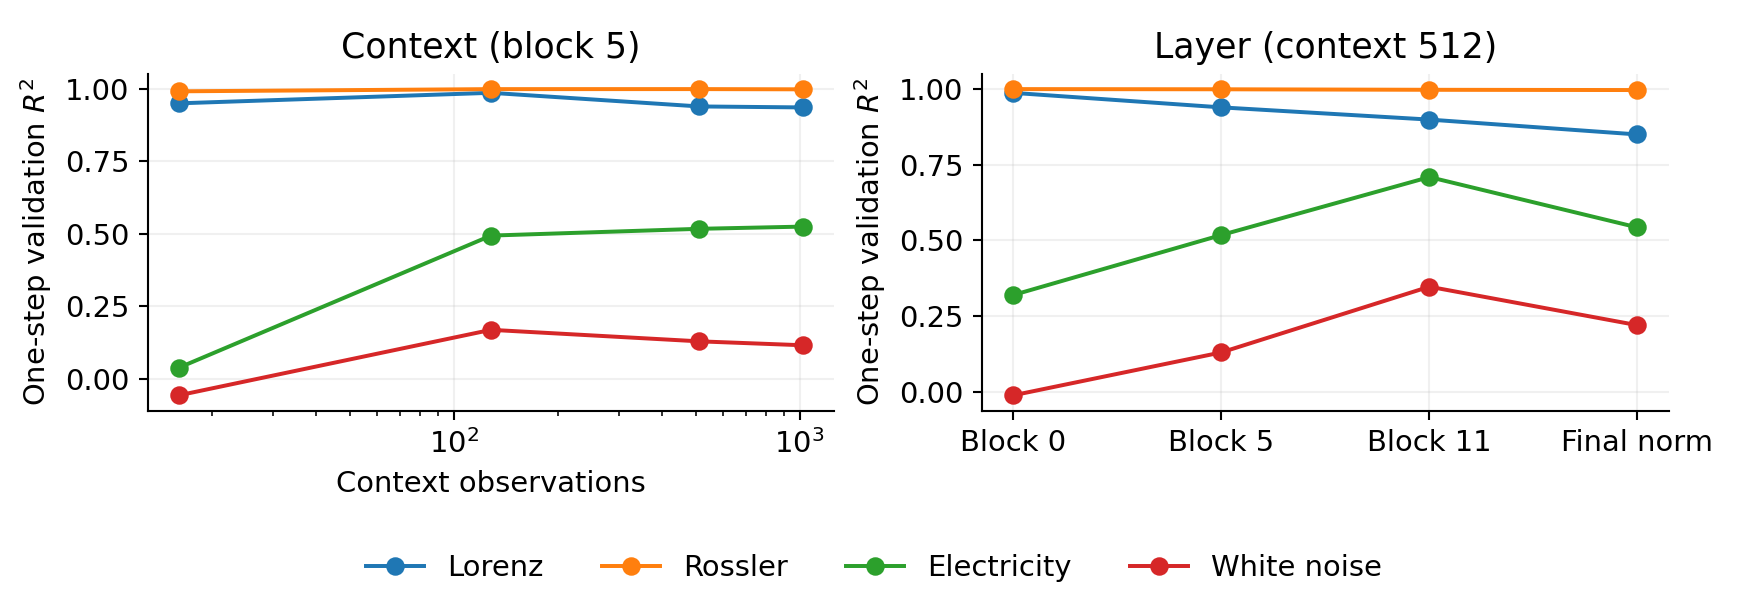
\includegraphics[width=.87\textwidth]{images/representation_controls.png}
\caption{One-step Ridge: block 0 is first, block 5 middle (6th of 12), block 11 last. Final norm follows the last block. Each condition predicts its own hidden target.}
\end{figure}
\small
Changing the encoder changes the target. Random-weight predictability does not measure raw-series forecasting accuracy.
\end{frame}

\subsection{Depth criterion}
\begin{frame}{Depth-control specificity}
The depth predictor learns $F_d(h_{5,t})\approx h_{6,t}$.
The declared comparison scores both predictors against $h_{5,t+1}$.
\[
 \Delta R^2=R^2(F_{\rm time})-R^2(F_d),\qquad
 \Delta\cos=\cos(F_{\rm time})-\cos(F_d).
\]
\begin{itemize}
\item H2 requires gains of at least 0.05 in both metrics and positive paired bootstrap lower bounds.
\item On white noise, even the constant training-target mean beats the depth map by 1.067 in $R^2$ and 0.183 in cosine.
\end{itemize}
\vspace{3mm}
The threshold can pass for a trivial temporal predictor. It does not establish meaningful temporal dynamics or show that depth prediction itself is difficult.
\end{frame}

\subsection{References}
\begin{frame}{Selected references and code}
\small
\begin{itemize}
\item Ansari et al. Chronos-2: From Univariate to Universal Forecasting, 2025.
\item Wili\'nski et al. Exploring Representations and Interventions in Time Series Foundation Models, 2025.
\item Yang et al. From Observations to States: Latent Time Series Forecasting, 2026.
\item Zhou et al. EIDOS: Latent-Space Predictive Learning for Time Series Foundation Models, 2026.
\item Chen et al. Neural Ordinary Differential Equations, 2018.
\item Gilpin. Chaos as an Interpretable Benchmark for Forecasting and Data-driven Modelling, 2021.
\end{itemize}
\vspace{2mm}
\scriptsize
\url{https://github.com/nikita-aleksandrov-wr/hidden-state-evolution-analysis}
\end{frame}

\end{document}
